\begin{pastexam}[label={px:ccu-113-csb-01}]{中正資工所乙組 113 學年度 第 5 題}
（單選，並說明理由）

(5\%) Given the following graph, please choose the edges in the spanning tree constructed by DFS.
Note that the starting node is node 1, and the node with a smaller ID will be visited first if there
is a tie.

\begin{center}
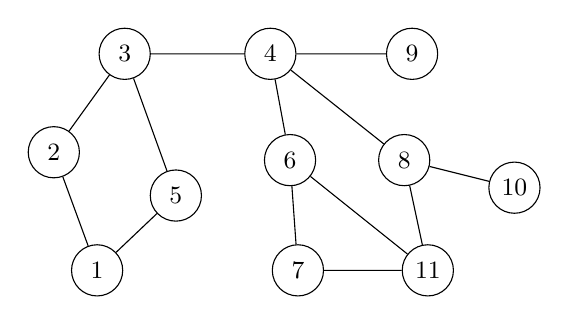
\begin{tikzpicture}[v/.style={circle,draw,minimum size=6.5mm,inner sep=0pt,font=\small}]
\node[v] (3) at (1.2,2.75) {3};
\node[v] (4) at (3.05,2.75) {4};
\node[v] (9) at (4.85,2.75) {9};
\node[v] (2) at (0.3,1.5) {2};
\node[v] (5) at (1.85,0.95) {5};
\node[v] (6) at (3.3,1.4) {6};
\node[v] (8) at (4.75,1.4) {8};
\node[v] (10) at (6.15,1.05) {10};
\node[v] (1) at (0.85,0) {1};
\node[v] (7) at (3.4,0) {7};
\node[v] (11) at (5.05,0) {11};
\draw (1)--(2) (2)--(3) (3)--(5) (5)--(1) (3)--(4) (4)--(9) (4)--(6) (4)--(8)
      (6)--(7) (6)--(11) (7)--(11) (8)--(10) (8)--(11);
\end{tikzpicture}
\end{center}

(a)~(1, 2), (2, 3), (3, 4), (3, 5), (4, 6), (4, 9), (6, 7), (7, 11), (8, 10), (8, 11)\\
(b)~(1, 2), (1, 5), (2, 3), (3, 4), (4, 6), (4, 8), (4, 9), (6, 7), (6, 11), (8, 10)\\
(c)~(1, 5), (2, 3), (3, 5), (3, 4), (4, 8), (4, 9), (6, 7), (7, 11), (8, 10), (8, 11)\\
(d)~None of them
\end{pastexam}

\begin{pastsoln}
答案是 (a)。

照資結書第~21.4~節的 DFS：從一個頂點出發，依編號由小到大看它的鄰居，遇到還沒拜訪的就立刻走
過去（遞迴），走不下去才退回上一個頂點繼續看下一個鄰居。 每次「走過去」用的那條邊就是 DFS 樹的
邊。 各頂點的鄰居（由小到大）：
\begin{center}
\small
\begin{tabular}{c|ccccccccccc}
頂點 & 1 & 2 & 3 & 4 & 5 & 6 & 7 & 8 & 9 & 10 & 11 \\ \hline
鄰居 & 2, 5 & 1, 3 & 2, 4, 5 & 3, 6, 8, 9 & 1, 3 & 4, 7, 11 & 6, 11 & 4, 10, 11 & 4 & 8 & 6, 7, 8 \\
\end{tabular}
\end{center}
追蹤（括號裡是當時的遞迴堆疊，最右邊是目前的頂點）：
\begin{enumerate}[itemsep=0pt]
\item 從 $1$ 開始。 $1$ 的第一個鄰居 $2$ 沒拜訪過，走 $(1, 2)$。 \hfill $(1, 2)$
\item $2$ 的鄰居 $1$ 已拜訪，$3$ 沒有，走 $(2, 3)$。 \hfill $(1, 2, 3)$
\item $3$ 的鄰居 $2$ 已拜訪，$4$ 沒有，走 $(3, 4)$。 \hfill $(1, 2, 3, 4)$
\item $4$ 的鄰居 $3$ 已拜訪，$6$ 沒有，走 $(4, 6)$。 \hfill $(1, 2, 3, 4, 6)$
\item $6$ 的鄰居 $4$ 已拜訪，$7$ 沒有，走 $(6, 7)$。 \hfill $(1, 2, 3, 4, 6, 7)$
\item $7$ 的鄰居 $6$ 已拜訪，$11$ 沒有，走 $(7, 11)$。 \hfill $(1, 2, 3, 4, 6, 7, 11)$
\item $11$ 的鄰居 $6$、$7$ 已拜訪，$8$ 沒有，走 $(11, 8)$。 \hfill $(1, 2, 3, 4, 6, 7, 11, 8)$
\item $8$ 的鄰居 $4$ 已拜訪，$10$ 沒有，走 $(8, 10)$。 $10$ 沒有其他鄰居，退回 $8$；$8$ 的鄰居 $11$
已拜訪，退回 $11$、$7$、$6$，都沒有新鄰居，退回 $4$。
\item $4$ 的下一個鄰居 $8$ 已拜訪，$9$ 沒有，走 $(4, 9)$。 退回 $4$、再退回 $3$。
\item $3$ 的下一個鄰居 $5$ 沒拜訪過，走 $(3, 5)$。 $5$ 的鄰居都拜訪過了，一路退回 $1$；$1$ 的下一個
鄰居 $5$ 已拜訪，結束。
\end{enumerate}
拜訪順序 $1, 2, 3, 4, 6, 7, 11, 8, 10, 9, 5$，樹邊共 $10$ 條（$11$ 個頂點的生成樹）：
\[
(1, 2), (2, 3), (3, 4), (3, 5), (4, 6), (4, 9), (6, 7), (7, 11), (8, 10), (8, 11),
\]
就是 (a)。 注意 $5$ 雖然是 $1$ 的鄰居，但等 DFS 退回 $1$ 時 $5$ 早就從 $3$ 走到了，所以樹邊是
$(3, 5)$ 不是 $(1, 5)$；$8$ 也是從 $11$ 走到的，不是從 $4$。

其他選項：
\begin{itemize}
\item (b) 有 $(1, 5)$、$(4, 8)$、$(6, 11)$，這是從 $1$ 出發的 \textbf{BFS} 樹：$1$ 一次把 $2$、$5$ 都
放進佇列，$4$ 一次把 $6$、$8$、$9$ 都放進去。 錯。
\item (c) 是鄰居改成\textbf{由大到小}看的 DFS 樹：$1 \to 5 \to 3 \to 4 \to 9$，退回 $4$ 後
$\to 8 \to 11 \to 7 \to 6$，再 $8 \to 10$，最後 $3 \to 2$。 和題目「編號小的先」相反。 錯。
\item (d)：(a) 正確，錯。
\end{itemize}
\end{pastsoln}
